\begin{frame}
	\frametitle{Testes Complementares}
		\framesubtitle{Espalhamento de valores dos vetores de características}
		\only<1>{
			\begin{multicols}{2}
				\begin{figure}[H]
					\centering
					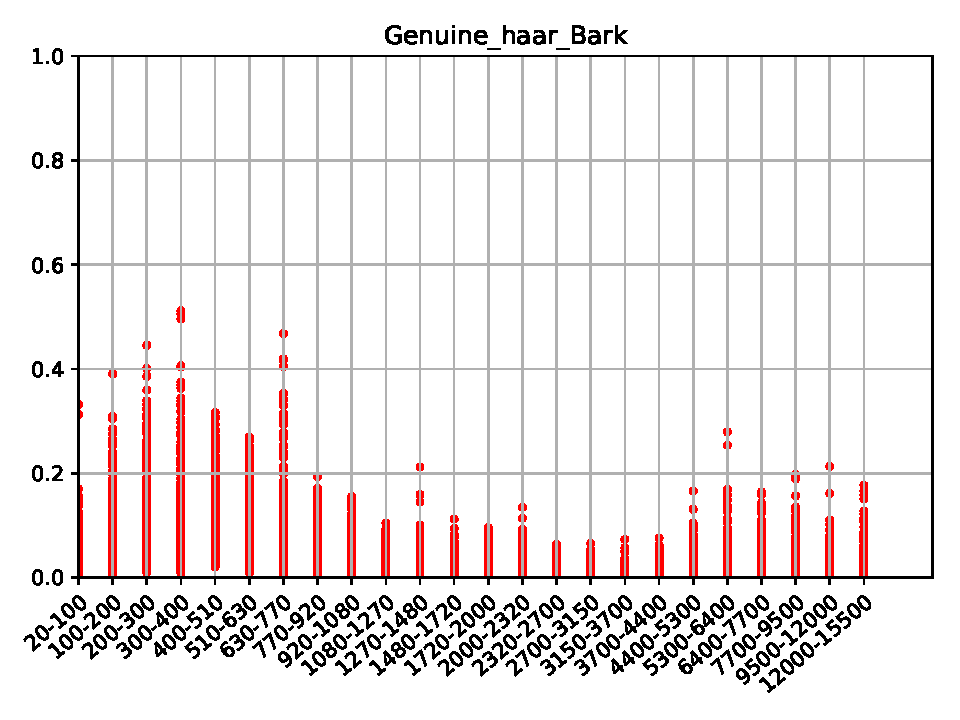
\includegraphics[scale=.38]{../monography/images/results/barkVersusMel/Genuine_haar_Bark.pdf}
					\caption{Gráfico de dispersão para os vetores de características \textit{genuínos} obtidos com \textit{Haar + BARK}. Eixos horizontais e verticais: Bandas de frequência em Hertz(Hz) e amplitudes, respectivamente.}
					\label{fig:livehaarbark}
				\end{figure}
				\begin{figure}[H]
					\centering
					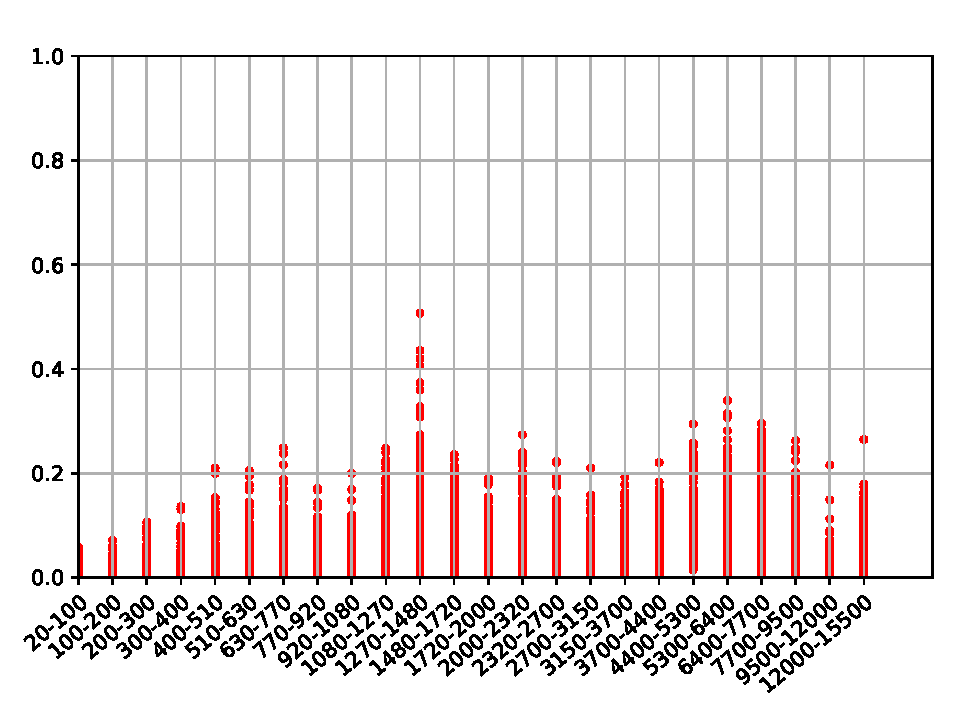
\includegraphics[scale=.38]{../monography/images/results/barkVersusMel/Spoofing_haar_Bark.pdf}
					\caption{Gráfico de dispersão para os vetores de características \textit{falseados} obtidos com \textit{Haar + BARK}. Eixos horizontais e verticais: Banda de frequência em Hertz(Hz) e amplitudes, respectivamente.}
					\label{fig:spoofinghaarbark}
				\end{figure}
			\end{multicols}
		}
		\only<2>{
			\begin{multicols}{2}
				\begin{figure}[H]
					\centering
					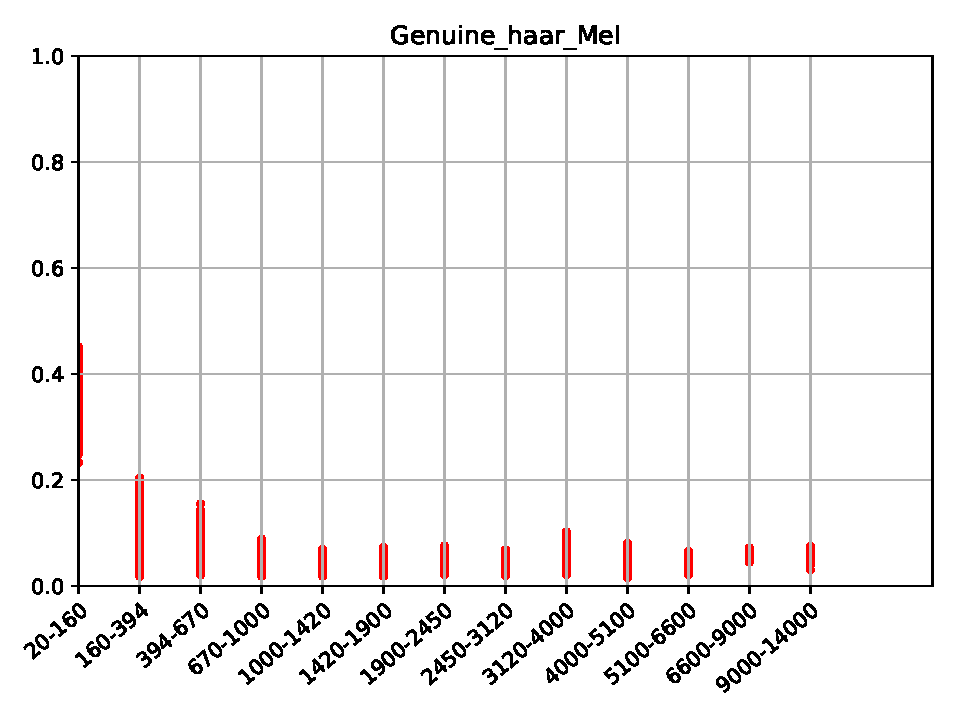
\includegraphics[scale=.38]{../monography/images/results/barkVersusMel/Genuine_haar_Mel.pdf}
					\caption{Gráfico de dispersão para vetores de características \textit{genuínos} obtidos com \textit{Haar + MEL}. Eixos horizontais e verticais: Bandas de frequência em Hertz(Hz) e amplitudes, respectivamente.}
					\label{fig:livehaarmel}
				\end{figure}
				\begin{figure}[H]
					\centering
					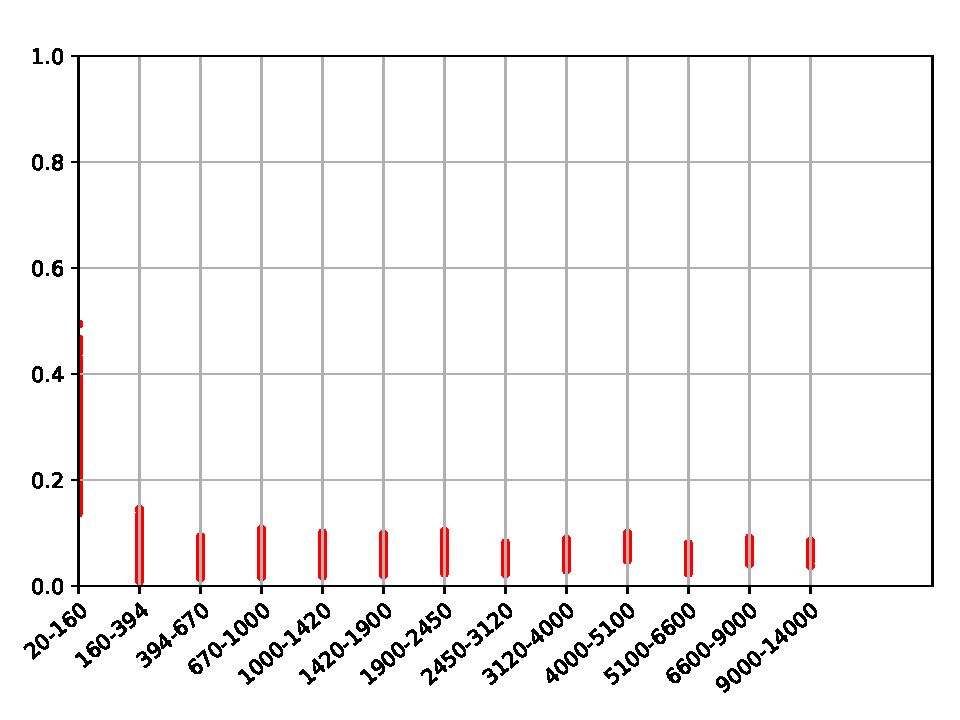
\includegraphics[scale=.38]{../monography/images/results/barkVersusMel/Spoofing_haar_Mel.pdf}
					\caption{Gráfico de dispersão para vetores de características \textit{falseados} obtidos com \textit{Haar + MEL}. Eixos horizontais e verticais: Bandas de frequência em Hertz(Hz) e amplitudes, respectivamente.}
					\label{fig:spoofinghaarmel}
				\end{figure}
			\end{multicols}
		}
\end{frame}